\documentclass[twoside]{article}

% Packages required by doxygen
\usepackage{fixltx2e}
\usepackage{calc}
\usepackage{doxygen}
\usepackage[export]{adjustbox} % also loads graphicx
\usepackage{graphicx}
\usepackage[utf8]{inputenc}
\usepackage{makeidx}
\usepackage{multicol}
\usepackage{multirow}
\PassOptionsToPackage{warn}{textcomp}
\usepackage{textcomp}
\usepackage[nointegrals]{wasysym}
\usepackage[table]{xcolor}

% Font selection
\usepackage[T1]{fontenc}
\usepackage[scaled=.90]{helvet}
\usepackage{courier}
\usepackage{amssymb}
\usepackage{sectsty}
\renewcommand{\familydefault}{\sfdefault}
\allsectionsfont{%
  \fontseries{bc}\selectfont%
  \color{darkgray}%
}
\renewcommand{\DoxyLabelFont}{%
  \fontseries{bc}\selectfont%
  \color{darkgray}%
}
\newcommand{\+}{\discretionary{\mbox{\scriptsize$\hookleftarrow$}}{}{}}

% Page & text layout
\usepackage{geometry}
\geometry{%
  a4paper,%
  top=2.5cm,%
  bottom=2.5cm,%
  left=2.5cm,%
  right=2.5cm%
}
\tolerance=750
\hfuzz=15pt
\hbadness=750
\setlength{\emergencystretch}{15pt}
\setlength{\parindent}{0cm}
\setlength{\parskip}{3ex plus 2ex minus 2ex}
\makeatletter
\renewcommand{\paragraph}{%
  \@startsection{paragraph}{4}{0ex}{-1.0ex}{1.0ex}{%
    \normalfont\normalsize\bfseries\SS@parafont%
  }%
}
\renewcommand{\subparagraph}{%
  \@startsection{subparagraph}{5}{0ex}{-1.0ex}{1.0ex}{%
    \normalfont\normalsize\bfseries\SS@subparafont%
  }%
}
\makeatother

% Headers & footers
\usepackage{fancyhdr}
\pagestyle{fancyplain}
\fancyhead[LE]{\fancyplain{}{\bfseries\thepage}}
\fancyhead[CE]{\fancyplain{}{}}
\fancyhead[RE]{\fancyplain{}{\bfseries\leftmark}}
\fancyhead[LO]{\fancyplain{}{\bfseries\rightmark}}
\fancyhead[CO]{\fancyplain{}{}}
\fancyhead[RO]{\fancyplain{}{\bfseries\thepage}}
\fancyfoot[LE]{\fancyplain{}{}}
\fancyfoot[CE]{\fancyplain{}{}}
\fancyfoot[RE]{\fancyplain{}{\bfseries\scriptsize Generated by Doxygen }}
\fancyfoot[LO]{\fancyplain{}{\bfseries\scriptsize Generated by Doxygen }}
\fancyfoot[CO]{\fancyplain{}{}}
\fancyfoot[RO]{\fancyplain{}{}}
\renewcommand{\footrulewidth}{0.4pt}
\renewcommand{\sectionmark}[1]{%
  \markright{\thesection\ #1}%
}

% Indices & bibliography
\usepackage{natbib}
\usepackage[titles]{tocloft}
\setcounter{tocdepth}{3}
\setcounter{secnumdepth}{5}
\makeindex

% Hyperlinks (required, but should be loaded last)
\usepackage{ifpdf}
\ifpdf
  \usepackage[pdftex,pagebackref=true]{hyperref}
\else
  \usepackage[ps2pdf,pagebackref=true]{hyperref}
\fi
\hypersetup{%
  colorlinks=true,%
  linkcolor=blue,%
  citecolor=blue,%
  unicode%
}

% Custom commands
\newcommand{\clearemptydoublepage}{%
  \newpage{\pagestyle{empty}\cleardoublepage}%
}

\usepackage{caption}
\captionsetup{labelsep=space,justification=centering,font={bf},singlelinecheck=off,skip=4pt,position=top}

%===== C O N T E N T S =====

\begin{document}

% Titlepage & ToC
\hypersetup{pageanchor=false,
             bookmarksnumbered=true,
             pdfencoding=unicode
            }
\pagenumbering{alph}
\begin{titlepage}
\vspace*{7cm}
\begin{center}%
{\Large P\+A01 -\/ Linked List }\\
\vspace*{1cm}
{\large Generated by Doxygen 1.8.12}\\
\end{center}
\end{titlepage}
\pagenumbering{roman}
\tableofcontents
\pagenumbering{arabic}
\hypersetup{pageanchor=true}

%--- Begin generated contents ---
\section{Hierarchical Index}
\section{Class Hierarchy}
This inheritance list is sorted roughly, but not completely, alphabetically\+:\begin{DoxyCompactList}
\item \contentsline{section}{Binary\+Node$<$ Item\+Type $>$}{\pageref{class_binary_node}}{}
\item \contentsline{section}{Binary\+Node\+Tree$<$ Item\+Type $>$}{\pageref{class_binary_node_tree}}{}
\begin{DoxyCompactList}
\item \contentsline{section}{Binary\+Search\+Tree$<$ Item\+Type $>$}{\pageref{class_binary_search_tree}}{}
\end{DoxyCompactList}
\end{DoxyCompactList}

\section{Class Index}
\subsection{Class List}
Here are the classes, structs, unions and interfaces with brief descriptions\+:\begin{DoxyCompactList}
\item\contentsline{section}{\hyperlink{class_linked_list}{Linked\+List$<$ Item\+Type $>$} }{\pageref{class_linked_list}}{}
\item\contentsline{section}{\hyperlink{class_list_interface}{List\+Interface$<$ Item\+Type $>$} }{\pageref{class_list_interface}}{}
\item\contentsline{section}{\hyperlink{class_node}{Node$<$ Item\+Type $>$} }{\pageref{class_node}}{}
\item\contentsline{section}{\hyperlink{class_precond_violated_except}{Precond\+Violated\+Except} }{\pageref{class_precond_violated_except}}{}
\end{DoxyCompactList}

\section{File Index}
\section{File List}
Here is a list of all documented files with brief descriptions\+:\begin{DoxyCompactList}
\item\contentsline{section}{\hyperlink{_binary_node_8cpp}{Binary\+Node.\+cpp} \\*Implementation file for the Binary Node class }{\pageref{_binary_node_8cpp}}{}
\item\contentsline{section}{\hyperlink{_binary_node_8h}{Binary\+Node.\+h} \\*Header file for the Binary Node class }{\pageref{_binary_node_8h}}{}
\item\contentsline{section}{\hyperlink{_binary_node_tree_8cpp}{Binary\+Node\+Tree.\+cpp} \\*Implementation file for the Binary Node Tree class }{\pageref{_binary_node_tree_8cpp}}{}
\item\contentsline{section}{\hyperlink{_binary_node_tree_8h}{Binary\+Node\+Tree.\+h} \\*Header file for the Binary Node Tree class }{\pageref{_binary_node_tree_8h}}{}
\item\contentsline{section}{\hyperlink{_binary_search_tree_8cpp}{Binary\+Search\+Tree.\+cpp} \\*Implementation file for the Binary Search Tree class }{\pageref{_binary_search_tree_8cpp}}{}
\item\contentsline{section}{\hyperlink{_binary_search_tree_8h}{Binary\+Search\+Tree.\+h} \\*Header file for the Binary Search Tree class }{\pageref{_binary_search_tree_8h}}{}
\item\contentsline{section}{\hyperlink{_p_a07_8cpp}{P\+A07.\+cpp} \\*Main driver for project 7 }{\pageref{_p_a07_8cpp}}{}
\item\contentsline{section}{\hyperlink{_red_black_tree_8cpp}{Red\+Black\+Tree.\+cpp} \\*Implementation file for the Red Black Tree class }{\pageref{_red_black_tree_8cpp}}{}
\item\contentsline{section}{\hyperlink{_red_black_tree_8h}{Red\+Black\+Tree.\+h} \\*Header file for the Red Black Tree class }{\pageref{_red_black_tree_8h}}{}
\end{DoxyCompactList}

\section{Class Documentation}
\hypertarget{class_linked_list}{}\subsection{Linked\+List$<$ Item\+Type $>$ Class Template Reference}
\label{class_linked_list}\index{Linked\+List$<$ Item\+Type $>$@{Linked\+List$<$ Item\+Type $>$}}
Inheritance diagram for Linked\+List$<$ Item\+Type $>$\+:\begin{figure}[H]
\begin{center}
\leavevmode
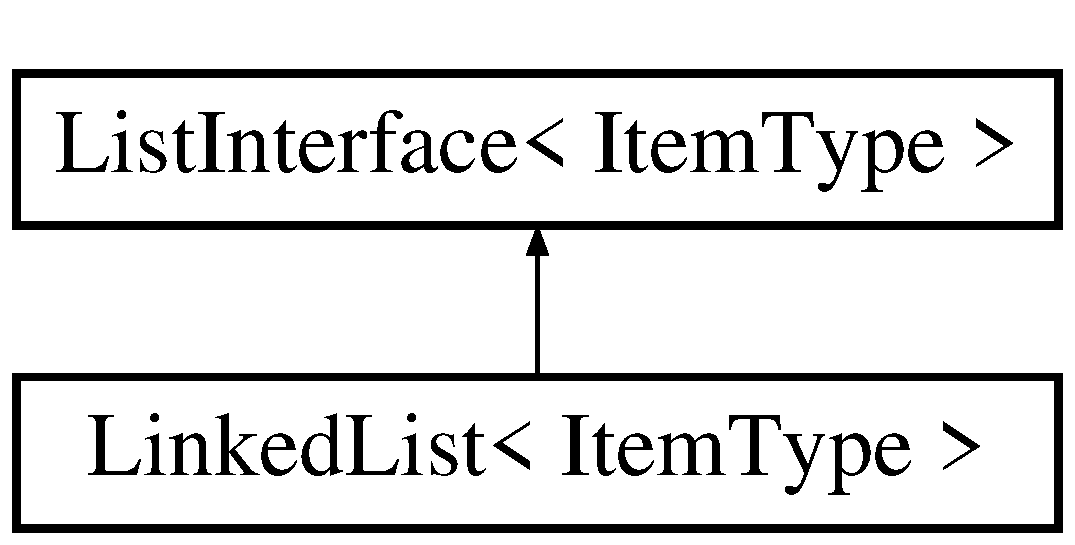
\includegraphics[height=2.000000cm]{class_linked_list}
\end{center}
\end{figure}
\subsubsection*{Public Member Functions}
\begin{DoxyCompactItemize}
\item 
\hypertarget{class_linked_list_a6f1443c6120352f1f5b6bd3c0d95e41e}{}\label{class_linked_list_a6f1443c6120352f1f5b6bd3c0d95e41e} 
{\bfseries Linked\+List} (const \hyperlink{class_linked_list}{Linked\+List}$<$ Item\+Type $>$ \&a\+List)
\item 
bool \hyperlink{class_linked_list_a008e916c3d51d28b4cc9c8cdf3e9d921}{is\+Empty} () const
\item 
int \hyperlink{class_linked_list_a61d045ef6008b494a1a516ecc992c0e7}{get\+Length} () const
\item 
bool \hyperlink{class_linked_list_ae8a19375505e87e2e4fc0e9b5afe4d4d}{insert} (int new\+Position, const Item\+Type \&new\+Entry)
\item 
bool \hyperlink{class_linked_list_a16a02716b5b2efb6fb1e3d18721b53e4}{remove} (int position)
\item 
void \hyperlink{class_linked_list_a7d1d9cf83eef67b6c4d700a3cc5970e1}{clear} ()
\item 
Item\+Type \hyperlink{class_linked_list_a341bfd7772c9d24d29eb7a7f3936915b}{get\+Entry} (int position) const  throw (\+Precond\+Violated\+Except)
\item 
void \hyperlink{class_linked_list_a3035f880c50e7d8f68e67c093d4607ca}{replace} (int position, const Item\+Type \&new\+Entry)  throw (\+Precond\+Violated\+Except)
\end{DoxyCompactItemize}
\subsubsection*{Private Member Functions}
\begin{DoxyCompactItemize}
\item 
\hypertarget{class_linked_list_ac707777d9e457c986eb18c1366efafd2}{}\label{class_linked_list_ac707777d9e457c986eb18c1366efafd2} 
\hyperlink{class_node}{Node}$<$ Item\+Type $>$ $\ast$ {\bfseries get\+Node\+At} (int position) const
\item 
\hypertarget{class_linked_list_ab09a3ae73c7fa669e0116bd510d55a9d}{}\label{class_linked_list_ab09a3ae73c7fa669e0116bd510d55a9d} 
\hyperlink{class_node}{Node}$<$ Item\+Type $>$ $\ast$ {\bfseries insert\+Node} (int position, \hyperlink{class_node}{Node}$<$ Item\+Type $>$ $\ast$new\+Node\+Ptr, \hyperlink{class_node}{Node}$<$ Item\+Type $>$ $\ast$sub\+Chain\+Ptr)
\end{DoxyCompactItemize}
\subsubsection*{Private Attributes}
\begin{DoxyCompactItemize}
\item 
\hypertarget{class_linked_list_ae59caadbc6814867c20aa78f1bc9a566}{}\label{class_linked_list_ae59caadbc6814867c20aa78f1bc9a566} 
\hyperlink{class_node}{Node}$<$ Item\+Type $>$ $\ast$ {\bfseries head\+Ptr}
\item 
\hypertarget{class_linked_list_a964b92cf1253774e9e35f331d5fb3490}{}\label{class_linked_list_a964b92cf1253774e9e35f331d5fb3490} 
int {\bfseries item\+Count}
\end{DoxyCompactItemize}


\subsubsection{Member Function Documentation}
\hypertarget{class_linked_list_a7d1d9cf83eef67b6c4d700a3cc5970e1}{}\label{class_linked_list_a7d1d9cf83eef67b6c4d700a3cc5970e1} 
\index{Linked\+List@{Linked\+List}!clear@{clear}}
\index{clear@{clear}!Linked\+List@{Linked\+List}}
\paragraph{\texorpdfstring{clear()}{clear()}}
{\footnotesize\ttfamily template$<$class Item\+Type $>$ \\
void \hyperlink{class_linked_list}{Linked\+List}$<$ Item\+Type $>$\+::clear (\begin{DoxyParamCaption}{ }\end{DoxyParamCaption})\hspace{0.3cm}{\ttfamily [virtual]}}

Removes all entries from this list. \begin{DoxyPostcond}{Postcondition}
List contains no entries and the count of items is 0. 
\end{DoxyPostcond}


Implements \hyperlink{class_list_interface_adfda414908b645bdf19bcab8269168b7}{List\+Interface$<$ Item\+Type $>$}.

\hypertarget{class_linked_list_a341bfd7772c9d24d29eb7a7f3936915b}{}\label{class_linked_list_a341bfd7772c9d24d29eb7a7f3936915b} 
\index{Linked\+List@{Linked\+List}!get\+Entry@{get\+Entry}}
\index{get\+Entry@{get\+Entry}!Linked\+List@{Linked\+List}}
\paragraph{\texorpdfstring{get\+Entry()}{getEntry()}}
{\footnotesize\ttfamily template$<$class Item\+Type $>$ \\
Item\+Type \hyperlink{class_linked_list}{Linked\+List}$<$ Item\+Type $>$\+::get\+Entry (\begin{DoxyParamCaption}\item[{int}]{position }\end{DoxyParamCaption}) const throw  \hyperlink{class_precond_violated_except}{Precond\+Violated\+Except}) \hspace{0.3cm}{\ttfamily [virtual]}}


\begin{DoxyExceptions}{Exceptions}
{\em \hyperlink{class_precond_violated_except}{Precond\+Violated\+Except}} & if position $<$ 1 or position $>$ \hyperlink{class_linked_list_a61d045ef6008b494a1a516ecc992c0e7}{get\+Length()}. \\
\hline
\end{DoxyExceptions}


Implements \hyperlink{class_list_interface_a86987f69e5056d287212ede41db1956a}{List\+Interface$<$ Item\+Type $>$}.

\hypertarget{class_linked_list_a61d045ef6008b494a1a516ecc992c0e7}{}\label{class_linked_list_a61d045ef6008b494a1a516ecc992c0e7} 
\index{Linked\+List@{Linked\+List}!get\+Length@{get\+Length}}
\index{get\+Length@{get\+Length}!Linked\+List@{Linked\+List}}
\paragraph{\texorpdfstring{get\+Length()}{getLength()}}
{\footnotesize\ttfamily template$<$class Item\+Type $>$ \\
int \hyperlink{class_linked_list}{Linked\+List}$<$ Item\+Type $>$\+::get\+Length (\begin{DoxyParamCaption}{ }\end{DoxyParamCaption}) const\hspace{0.3cm}{\ttfamily [virtual]}}

Gets the current number of entries in this list. \begin{DoxyReturn}{Returns}
The integer number of entries currently in the list. 
\end{DoxyReturn}


Implements \hyperlink{class_list_interface_afc85695d4137f1e29ff02e179c9f3221}{List\+Interface$<$ Item\+Type $>$}.

\hypertarget{class_linked_list_ae8a19375505e87e2e4fc0e9b5afe4d4d}{}\label{class_linked_list_ae8a19375505e87e2e4fc0e9b5afe4d4d} 
\index{Linked\+List@{Linked\+List}!insert@{insert}}
\index{insert@{insert}!Linked\+List@{Linked\+List}}
\paragraph{\texorpdfstring{insert()}{insert()}}
{\footnotesize\ttfamily template$<$class Item\+Type $>$ \\
bool \hyperlink{class_linked_list}{Linked\+List}$<$ Item\+Type $>$\+::insert (\begin{DoxyParamCaption}\item[{int}]{new\+Position,  }\item[{const Item\+Type \&}]{new\+Entry }\end{DoxyParamCaption})\hspace{0.3cm}{\ttfamily [virtual]}}

Inserts an entry into this list at a given position. \begin{DoxyPrecond}{Precondition}
None. 
\end{DoxyPrecond}
\begin{DoxyPostcond}{Postcondition}
If 1 $<$= position $<$= \hyperlink{class_linked_list_a61d045ef6008b494a1a516ecc992c0e7}{get\+Length()} + 1 and the insertion is successful, new\+Entry is at the given position in the list, other entries are renumbered accordingly, and the returned value is true. 
\end{DoxyPostcond}

\begin{DoxyParams}{Parameters}
{\em new\+Position} & The list position at which to insert new\+Entry. \\
\hline
{\em new\+Entry} & The entry to insert into the list. \\
\hline
\end{DoxyParams}
\begin{DoxyReturn}{Returns}
True if insertion is successful, or false if not. 
\end{DoxyReturn}


Implements \hyperlink{class_list_interface_a5b2f86954a86172699a3495982c38e77}{List\+Interface$<$ Item\+Type $>$}.

\hypertarget{class_linked_list_a008e916c3d51d28b4cc9c8cdf3e9d921}{}\label{class_linked_list_a008e916c3d51d28b4cc9c8cdf3e9d921} 
\index{Linked\+List@{Linked\+List}!is\+Empty@{is\+Empty}}
\index{is\+Empty@{is\+Empty}!Linked\+List@{Linked\+List}}
\paragraph{\texorpdfstring{is\+Empty()}{isEmpty()}}
{\footnotesize\ttfamily template$<$class Item\+Type $>$ \\
bool \hyperlink{class_linked_list}{Linked\+List}$<$ Item\+Type $>$\+::is\+Empty (\begin{DoxyParamCaption}{ }\end{DoxyParamCaption}) const\hspace{0.3cm}{\ttfamily [virtual]}}

Sees whether this list is empty. \begin{DoxyReturn}{Returns}
True if the list is empty; otherwise returns false. 
\end{DoxyReturn}


Implements \hyperlink{class_list_interface_a924f91e7f81d7dcd3fda79bbcc671394}{List\+Interface$<$ Item\+Type $>$}.

\hypertarget{class_linked_list_a16a02716b5b2efb6fb1e3d18721b53e4}{}\label{class_linked_list_a16a02716b5b2efb6fb1e3d18721b53e4} 
\index{Linked\+List@{Linked\+List}!remove@{remove}}
\index{remove@{remove}!Linked\+List@{Linked\+List}}
\paragraph{\texorpdfstring{remove()}{remove()}}
{\footnotesize\ttfamily template$<$class Item\+Type $>$ \\
bool \hyperlink{class_linked_list}{Linked\+List}$<$ Item\+Type $>$\+::remove (\begin{DoxyParamCaption}\item[{int}]{position }\end{DoxyParamCaption})\hspace{0.3cm}{\ttfamily [virtual]}}

Removes the entry at a given position from this list. \begin{DoxyPrecond}{Precondition}
None. 
\end{DoxyPrecond}
\begin{DoxyPostcond}{Postcondition}
If 1 $<$= position $<$= \hyperlink{class_linked_list_a61d045ef6008b494a1a516ecc992c0e7}{get\+Length()} and the removal is successful, the entry at the given position in the list is removed, other items are renumbered accordingly, and the returned value is true. 
\end{DoxyPostcond}

\begin{DoxyParams}{Parameters}
{\em position} & The list position of the entry to remove. \\
\hline
\end{DoxyParams}
\begin{DoxyReturn}{Returns}
True if removal is successful, or false if not. 
\end{DoxyReturn}


Implements \hyperlink{class_list_interface_a5543002ec0d64bd2a63f3732f437af65}{List\+Interface$<$ Item\+Type $>$}.

\hypertarget{class_linked_list_a3035f880c50e7d8f68e67c093d4607ca}{}\label{class_linked_list_a3035f880c50e7d8f68e67c093d4607ca} 
\index{Linked\+List@{Linked\+List}!replace@{replace}}
\index{replace@{replace}!Linked\+List@{Linked\+List}}
\paragraph{\texorpdfstring{replace()}{replace()}}
{\footnotesize\ttfamily template$<$class Item\+Type $>$ \\
void \hyperlink{class_linked_list}{Linked\+List}$<$ Item\+Type $>$\+::replace (\begin{DoxyParamCaption}\item[{int}]{position,  }\item[{const Item\+Type \&}]{new\+Entry }\end{DoxyParamCaption}) throw  \hyperlink{class_precond_violated_except}{Precond\+Violated\+Except}) \hspace{0.3cm}{\ttfamily [virtual]}}


\begin{DoxyExceptions}{Exceptions}
{\em \hyperlink{class_precond_violated_except}{Precond\+Violated\+Except}} & if position $<$ 1 or position $>$ \hyperlink{class_linked_list_a61d045ef6008b494a1a516ecc992c0e7}{get\+Length()}. \\
\hline
\end{DoxyExceptions}


Implements \hyperlink{class_list_interface_aae877a56b7b9f5f526c37a00e234fad1}{List\+Interface$<$ Item\+Type $>$}.



The documentation for this class was generated from the following files\+:\begin{DoxyCompactItemize}
\item 
\hyperlink{_linked_list_8h}{Linked\+List.\+h}\item 
\hyperlink{_linked_list_8cpp}{Linked\+List.\+cpp}\end{DoxyCompactItemize}

\hypertarget{class_list_interface}{}\subsection{List\+Interface$<$ Item\+Type $>$ Class Template Reference}
\label{class_list_interface}\index{List\+Interface$<$ Item\+Type $>$@{List\+Interface$<$ Item\+Type $>$}}
Inheritance diagram for List\+Interface$<$ Item\+Type $>$\+:\begin{figure}[H]
\begin{center}
\leavevmode
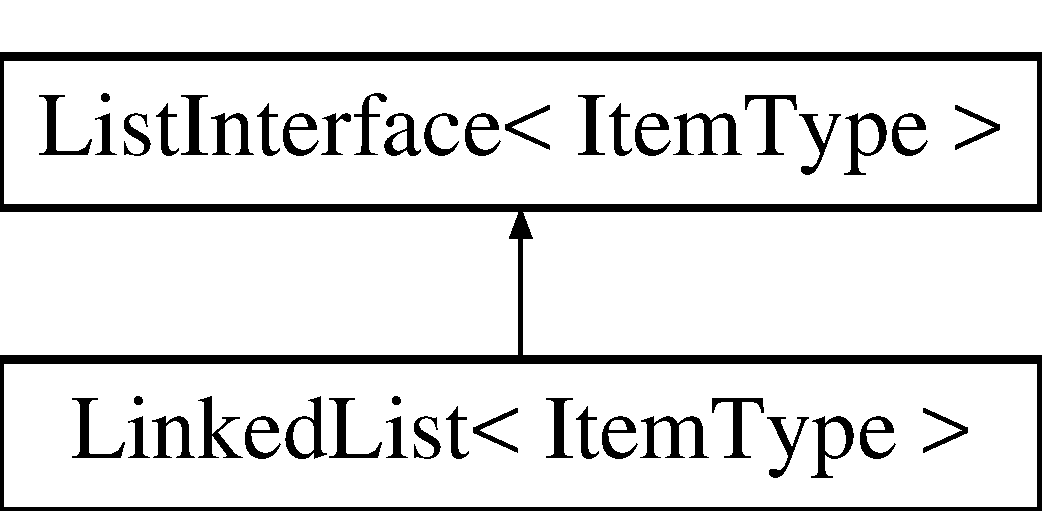
\includegraphics[height=2.000000cm]{class_list_interface}
\end{center}
\end{figure}
\subsubsection*{Public Member Functions}
\begin{DoxyCompactItemize}
\item 
virtual bool \hyperlink{class_list_interface_a924f91e7f81d7dcd3fda79bbcc671394}{is\+Empty} () const =0
\item 
virtual int \hyperlink{class_list_interface_afc85695d4137f1e29ff02e179c9f3221}{get\+Length} () const =0
\item 
virtual bool \hyperlink{class_list_interface_a5b2f86954a86172699a3495982c38e77}{insert} (int new\+Position, const Item\+Type \&new\+Entry)=0
\item 
virtual bool \hyperlink{class_list_interface_a5543002ec0d64bd2a63f3732f437af65}{remove} (int position)=0
\item 
virtual void \hyperlink{class_list_interface_adfda414908b645bdf19bcab8269168b7}{clear} ()=0
\item 
virtual Item\+Type \hyperlink{class_list_interface_a86987f69e5056d287212ede41db1956a}{get\+Entry} (int position) const =0
\item 
virtual void \hyperlink{class_list_interface_aae877a56b7b9f5f526c37a00e234fad1}{replace} (int position, const Item\+Type \&new\+Entry)=0
\end{DoxyCompactItemize}


\subsubsection{Member Function Documentation}
\hypertarget{class_list_interface_adfda414908b645bdf19bcab8269168b7}{}\label{class_list_interface_adfda414908b645bdf19bcab8269168b7} 
\index{List\+Interface@{List\+Interface}!clear@{clear}}
\index{clear@{clear}!List\+Interface@{List\+Interface}}
\paragraph{\texorpdfstring{clear()}{clear()}}
{\footnotesize\ttfamily template$<$class Item\+Type $>$ \\
virtual void \hyperlink{class_list_interface}{List\+Interface}$<$ Item\+Type $>$\+::clear (\begin{DoxyParamCaption}{ }\end{DoxyParamCaption})\hspace{0.3cm}{\ttfamily [pure virtual]}}

Removes all entries from this list. \begin{DoxyPostcond}{Postcondition}
List contains no entries and the count of items is 0. 
\end{DoxyPostcond}


Implemented in \hyperlink{class_linked_list_a7d1d9cf83eef67b6c4d700a3cc5970e1}{Linked\+List$<$ Item\+Type $>$}.

\hypertarget{class_list_interface_a86987f69e5056d287212ede41db1956a}{}\label{class_list_interface_a86987f69e5056d287212ede41db1956a} 
\index{List\+Interface@{List\+Interface}!get\+Entry@{get\+Entry}}
\index{get\+Entry@{get\+Entry}!List\+Interface@{List\+Interface}}
\paragraph{\texorpdfstring{get\+Entry()}{getEntry()}}
{\footnotesize\ttfamily template$<$class Item\+Type $>$ \\
virtual Item\+Type \hyperlink{class_list_interface}{List\+Interface}$<$ Item\+Type $>$\+::get\+Entry (\begin{DoxyParamCaption}\item[{int}]{position }\end{DoxyParamCaption}) const\hspace{0.3cm}{\ttfamily [pure virtual]}}

Gets the entry at the given position in this list. \begin{DoxyPrecond}{Precondition}
1 $<$= position $<$= \hyperlink{class_list_interface_afc85695d4137f1e29ff02e179c9f3221}{get\+Length()}. 
\end{DoxyPrecond}
\begin{DoxyPostcond}{Postcondition}
The desired entry has been returned. 
\end{DoxyPostcond}

\begin{DoxyParams}{Parameters}
{\em position} & The list position of the desired entry. \\
\hline
\end{DoxyParams}
\begin{DoxyReturn}{Returns}
The entry at the given position. 
\end{DoxyReturn}


Implemented in \hyperlink{class_linked_list_a341bfd7772c9d24d29eb7a7f3936915b}{Linked\+List$<$ Item\+Type $>$}.

\hypertarget{class_list_interface_afc85695d4137f1e29ff02e179c9f3221}{}\label{class_list_interface_afc85695d4137f1e29ff02e179c9f3221} 
\index{List\+Interface@{List\+Interface}!get\+Length@{get\+Length}}
\index{get\+Length@{get\+Length}!List\+Interface@{List\+Interface}}
\paragraph{\texorpdfstring{get\+Length()}{getLength()}}
{\footnotesize\ttfamily template$<$class Item\+Type $>$ \\
virtual int \hyperlink{class_list_interface}{List\+Interface}$<$ Item\+Type $>$\+::get\+Length (\begin{DoxyParamCaption}{ }\end{DoxyParamCaption}) const\hspace{0.3cm}{\ttfamily [pure virtual]}}

Gets the current number of entries in this list. \begin{DoxyReturn}{Returns}
The integer number of entries currently in the list. 
\end{DoxyReturn}


Implemented in \hyperlink{class_linked_list_a61d045ef6008b494a1a516ecc992c0e7}{Linked\+List$<$ Item\+Type $>$}.

\hypertarget{class_list_interface_a5b2f86954a86172699a3495982c38e77}{}\label{class_list_interface_a5b2f86954a86172699a3495982c38e77} 
\index{List\+Interface@{List\+Interface}!insert@{insert}}
\index{insert@{insert}!List\+Interface@{List\+Interface}}
\paragraph{\texorpdfstring{insert()}{insert()}}
{\footnotesize\ttfamily template$<$class Item\+Type $>$ \\
virtual bool \hyperlink{class_list_interface}{List\+Interface}$<$ Item\+Type $>$\+::insert (\begin{DoxyParamCaption}\item[{int}]{new\+Position,  }\item[{const Item\+Type \&}]{new\+Entry }\end{DoxyParamCaption})\hspace{0.3cm}{\ttfamily [pure virtual]}}

Inserts an entry into this list at a given position. \begin{DoxyPrecond}{Precondition}
None. 
\end{DoxyPrecond}
\begin{DoxyPostcond}{Postcondition}
If 1 $<$= position $<$= \hyperlink{class_list_interface_afc85695d4137f1e29ff02e179c9f3221}{get\+Length()} + 1 and the insertion is successful, new\+Entry is at the given position in the list, other entries are renumbered accordingly, and the returned value is true. 
\end{DoxyPostcond}

\begin{DoxyParams}{Parameters}
{\em new\+Position} & The list position at which to insert new\+Entry. \\
\hline
{\em new\+Entry} & The entry to insert into the list. \\
\hline
\end{DoxyParams}
\begin{DoxyReturn}{Returns}
True if insertion is successful, or false if not. 
\end{DoxyReturn}


Implemented in \hyperlink{class_linked_list_ae8a19375505e87e2e4fc0e9b5afe4d4d}{Linked\+List$<$ Item\+Type $>$}.

\hypertarget{class_list_interface_a924f91e7f81d7dcd3fda79bbcc671394}{}\label{class_list_interface_a924f91e7f81d7dcd3fda79bbcc671394} 
\index{List\+Interface@{List\+Interface}!is\+Empty@{is\+Empty}}
\index{is\+Empty@{is\+Empty}!List\+Interface@{List\+Interface}}
\paragraph{\texorpdfstring{is\+Empty()}{isEmpty()}}
{\footnotesize\ttfamily template$<$class Item\+Type $>$ \\
virtual bool \hyperlink{class_list_interface}{List\+Interface}$<$ Item\+Type $>$\+::is\+Empty (\begin{DoxyParamCaption}{ }\end{DoxyParamCaption}) const\hspace{0.3cm}{\ttfamily [pure virtual]}}

Sees whether this list is empty. \begin{DoxyReturn}{Returns}
True if the list is empty; otherwise returns false. 
\end{DoxyReturn}


Implemented in \hyperlink{class_linked_list_a008e916c3d51d28b4cc9c8cdf3e9d921}{Linked\+List$<$ Item\+Type $>$}.

\hypertarget{class_list_interface_a5543002ec0d64bd2a63f3732f437af65}{}\label{class_list_interface_a5543002ec0d64bd2a63f3732f437af65} 
\index{List\+Interface@{List\+Interface}!remove@{remove}}
\index{remove@{remove}!List\+Interface@{List\+Interface}}
\paragraph{\texorpdfstring{remove()}{remove()}}
{\footnotesize\ttfamily template$<$class Item\+Type $>$ \\
virtual bool \hyperlink{class_list_interface}{List\+Interface}$<$ Item\+Type $>$\+::remove (\begin{DoxyParamCaption}\item[{int}]{position }\end{DoxyParamCaption})\hspace{0.3cm}{\ttfamily [pure virtual]}}

Removes the entry at a given position from this list. \begin{DoxyPrecond}{Precondition}
None. 
\end{DoxyPrecond}
\begin{DoxyPostcond}{Postcondition}
If 1 $<$= position $<$= \hyperlink{class_list_interface_afc85695d4137f1e29ff02e179c9f3221}{get\+Length()} and the removal is successful, the entry at the given position in the list is removed, other items are renumbered accordingly, and the returned value is true. 
\end{DoxyPostcond}

\begin{DoxyParams}{Parameters}
{\em position} & The list position of the entry to remove. \\
\hline
\end{DoxyParams}
\begin{DoxyReturn}{Returns}
True if removal is successful, or false if not. 
\end{DoxyReturn}


Implemented in \hyperlink{class_linked_list_a16a02716b5b2efb6fb1e3d18721b53e4}{Linked\+List$<$ Item\+Type $>$}.

\hypertarget{class_list_interface_aae877a56b7b9f5f526c37a00e234fad1}{}\label{class_list_interface_aae877a56b7b9f5f526c37a00e234fad1} 
\index{List\+Interface@{List\+Interface}!replace@{replace}}
\index{replace@{replace}!List\+Interface@{List\+Interface}}
\paragraph{\texorpdfstring{replace()}{replace()}}
{\footnotesize\ttfamily template$<$class Item\+Type $>$ \\
virtual void \hyperlink{class_list_interface}{List\+Interface}$<$ Item\+Type $>$\+::replace (\begin{DoxyParamCaption}\item[{int}]{position,  }\item[{const Item\+Type \&}]{new\+Entry }\end{DoxyParamCaption})\hspace{0.3cm}{\ttfamily [pure virtual]}}

Replaces the entry at the given position in this list. \begin{DoxyPrecond}{Precondition}
1 $<$= position $<$= \hyperlink{class_list_interface_afc85695d4137f1e29ff02e179c9f3221}{get\+Length()}. 
\end{DoxyPrecond}
\begin{DoxyPostcond}{Postcondition}
The entry at the given position is new\+Entry. 
\end{DoxyPostcond}

\begin{DoxyParams}{Parameters}
{\em position} & The list position of the entry to replace. \\
\hline
{\em new\+Entry} & The replacement entry. \\
\hline
\end{DoxyParams}


Implemented in \hyperlink{class_linked_list_a3035f880c50e7d8f68e67c093d4607ca}{Linked\+List$<$ Item\+Type $>$}.



The documentation for this class was generated from the following file\+:\begin{DoxyCompactItemize}
\item 
\hyperlink{_list_interface_8h}{List\+Interface.\+h}\end{DoxyCompactItemize}

\hypertarget{class_node}{}\subsection{Node$<$ Item\+Type $>$ Class Template Reference}
\label{class_node}\index{Node$<$ Item\+Type $>$@{Node$<$ Item\+Type $>$}}
\subsubsection*{Public Member Functions}
\begin{DoxyCompactItemize}
\item 
\hyperlink{class_node_a627e94f4fba0e73c546e0fb2a7266f36}{Node} ()
\begin{DoxyCompactList}\small\item\em Default constructor for the class. \end{DoxyCompactList}\item 
\hyperlink{class_node_a0288598fcb0244739ce95099c26250ae}{Node} (const Item\+Type \&an\+Item)
\begin{DoxyCompactList}\small\item\em Copy constructor for the class. \end{DoxyCompactList}\item 
\hypertarget{class_node_adf98d3f9b7227622cb5a0fdd7e8f0b18}{}\label{class_node_adf98d3f9b7227622cb5a0fdd7e8f0b18} 
\hyperlink{class_node_adf98d3f9b7227622cb5a0fdd7e8f0b18}{Node} (const Item\+Type \&an\+Item, \hyperlink{class_node}{Node}$<$ Item\+Type $>$ $\ast$next\+Node\+Ptr)
\begin{DoxyCompactList}\small\item\em Constructor for the class. \end{DoxyCompactList}\item 
void \hyperlink{class_node_ab4ceecdecc5df799011de486b9f54974}{set\+Item} (const Item\+Type \&an\+Item)
\begin{DoxyCompactList}\small\item\em set\+Item function \end{DoxyCompactList}\item 
void \hyperlink{class_node_a01c1a66d4e39f5b149e090413deb4633}{set\+Next} (\hyperlink{class_node}{Node}$<$ Item\+Type $>$ $\ast$next\+Node\+Ptr)
\begin{DoxyCompactList}\small\item\em set\+Next function \end{DoxyCompactList}\item 
Item\+Type \hyperlink{class_node_a6c08caef312b6f2f69b5e090cf047514}{get\+Item} () const
\begin{DoxyCompactList}\small\item\em get\+Item function \end{DoxyCompactList}\item 
\hyperlink{class_node}{Node}$<$ Item\+Type $>$ $\ast$ \hyperlink{class_node_a3eb0c96e03a3fd46ea1cff4c305bbedd}{get\+Next} () const
\begin{DoxyCompactList}\small\item\em get\+Next function \end{DoxyCompactList}\end{DoxyCompactItemize}
\subsubsection*{Private Attributes}
\begin{DoxyCompactItemize}
\item 
\hypertarget{class_node_a73e84414314067aa019ba6afb06190bd}{}\label{class_node_a73e84414314067aa019ba6afb06190bd} 
Item\+Type {\bfseries item}
\item 
\hypertarget{class_node_ad11288556b42a32b4f46ed955b7c31fd}{}\label{class_node_ad11288556b42a32b4f46ed955b7c31fd} 
\hyperlink{class_node}{Node}$<$ Item\+Type $>$ $\ast$ {\bfseries next}
\end{DoxyCompactItemize}


\subsubsection{Constructor \& Destructor Documentation}
\hypertarget{class_node_a627e94f4fba0e73c546e0fb2a7266f36}{}\label{class_node_a627e94f4fba0e73c546e0fb2a7266f36} 
\index{Node@{Node}!Node@{Node}}
\index{Node@{Node}!Node@{Node}}
\paragraph{\texorpdfstring{Node()}{Node()}\hspace{0.1cm}{\footnotesize\ttfamily [1/2]}}
{\footnotesize\ttfamily template$<$class Item\+Type $>$ \\
\hyperlink{class_node}{Node}$<$ Item\+Type $>$\+::\hyperlink{class_node}{Node} (\begin{DoxyParamCaption}{ }\end{DoxyParamCaption})}



Default constructor for the class. 

constructs the class \hypertarget{class_node_a0288598fcb0244739ce95099c26250ae}{}\label{class_node_a0288598fcb0244739ce95099c26250ae} 
\index{Node@{Node}!Node@{Node}}
\index{Node@{Node}!Node@{Node}}
\paragraph{\texorpdfstring{Node()}{Node()}\hspace{0.1cm}{\footnotesize\ttfamily [2/2]}}
{\footnotesize\ttfamily template$<$class Item\+Type $>$ \\
\hyperlink{class_node}{Node}$<$ Item\+Type $>$\+::\hyperlink{class_node}{Node} (\begin{DoxyParamCaption}\item[{const Item\+Type \&}]{an\+Item }\end{DoxyParamCaption})}



Copy constructor for the class. 

constructs the class using a previously constructed reference 

\subsubsection{Member Function Documentation}
\hypertarget{class_node_a6c08caef312b6f2f69b5e090cf047514}{}\label{class_node_a6c08caef312b6f2f69b5e090cf047514} 
\index{Node@{Node}!get\+Item@{get\+Item}}
\index{get\+Item@{get\+Item}!Node@{Node}}
\paragraph{\texorpdfstring{get\+Item()}{getItem()}}
{\footnotesize\ttfamily template$<$class Item\+Type $>$ \\
Item\+Type \hyperlink{class_node}{Node}$<$ Item\+Type $>$\+::get\+Item (\begin{DoxyParamCaption}{ }\end{DoxyParamCaption}) const}



get\+Item function 

returns current item \hypertarget{class_node_a3eb0c96e03a3fd46ea1cff4c305bbedd}{}\label{class_node_a3eb0c96e03a3fd46ea1cff4c305bbedd} 
\index{Node@{Node}!get\+Next@{get\+Next}}
\index{get\+Next@{get\+Next}!Node@{Node}}
\paragraph{\texorpdfstring{get\+Next()}{getNext()}}
{\footnotesize\ttfamily template$<$class Item\+Type $>$ \\
\hyperlink{class_node}{Node}$<$ Item\+Type $>$ $\ast$ \hyperlink{class_node}{Node}$<$ Item\+Type $>$\+::get\+Next (\begin{DoxyParamCaption}{ }\end{DoxyParamCaption}) const}



get\+Next function 

returns next item \hypertarget{class_node_ab4ceecdecc5df799011de486b9f54974}{}\label{class_node_ab4ceecdecc5df799011de486b9f54974} 
\index{Node@{Node}!set\+Item@{set\+Item}}
\index{set\+Item@{set\+Item}!Node@{Node}}
\paragraph{\texorpdfstring{set\+Item()}{setItem()}}
{\footnotesize\ttfamily template$<$class Item\+Type $>$ \\
void \hyperlink{class_node}{Node}$<$ Item\+Type $>$\+::set\+Item (\begin{DoxyParamCaption}\item[{const Item\+Type \&}]{an\+Item }\end{DoxyParamCaption})}



set\+Item function 

Sets the current item to another item \hypertarget{class_node_a01c1a66d4e39f5b149e090413deb4633}{}\label{class_node_a01c1a66d4e39f5b149e090413deb4633} 
\index{Node@{Node}!set\+Next@{set\+Next}}
\index{set\+Next@{set\+Next}!Node@{Node}}
\paragraph{\texorpdfstring{set\+Next()}{setNext()}}
{\footnotesize\ttfamily template$<$class Item\+Type $>$ \\
void \hyperlink{class_node}{Node}$<$ Item\+Type $>$\+::set\+Next (\begin{DoxyParamCaption}\item[{\hyperlink{class_node}{Node}$<$ Item\+Type $>$ $\ast$}]{next\+Node\+Ptr }\end{DoxyParamCaption})}



set\+Next function 

Sets the next item to an item 

The documentation for this class was generated from the following files\+:\begin{DoxyCompactItemize}
\item 
\hyperlink{_node_8h}{Node.\+h}\item 
\hyperlink{_node_8cpp}{Node.\+cpp}\end{DoxyCompactItemize}

\hypertarget{class_precond_violated_except}{}\subsection{Precond\+Violated\+Except Class Reference}
\label{class_precond_violated_except}\index{Precond\+Violated\+Except@{Precond\+Violated\+Except}}
Inheritance diagram for Precond\+Violated\+Except\+:\begin{figure}[H]
\begin{center}
\leavevmode
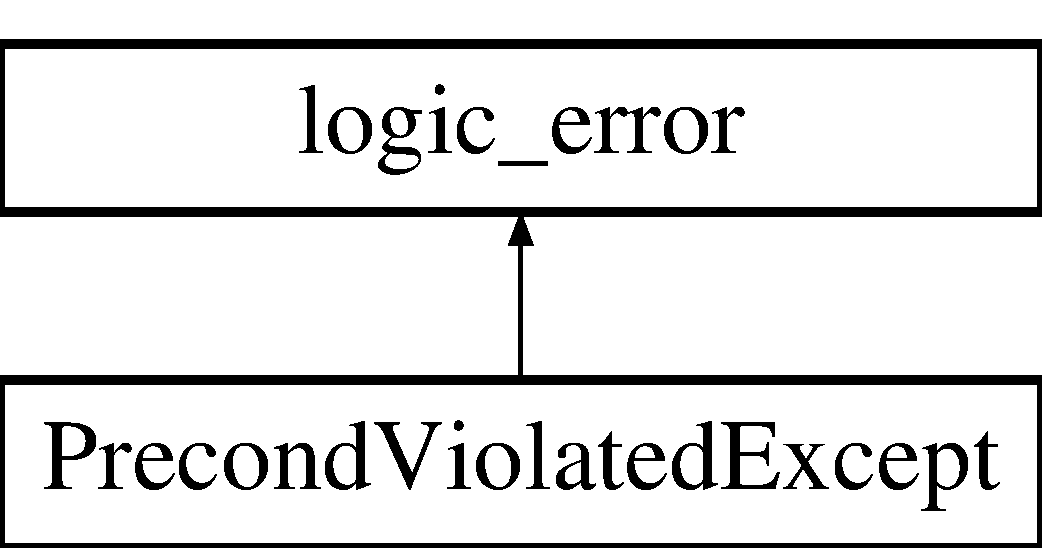
\includegraphics[height=2.000000cm]{class_precond_violated_except}
\end{center}
\end{figure}
\subsubsection*{Public Member Functions}
\begin{DoxyCompactItemize}
\item 
\hypertarget{class_precond_violated_except_a13c9075198f291ffc9a74c0c9b787ecf}{}\label{class_precond_violated_except_a13c9075198f291ffc9a74c0c9b787ecf} 
{\bfseries Precond\+Violated\+Except} (const std\+::string \&message=\char`\"{}\char`\"{})
\end{DoxyCompactItemize}


The documentation for this class was generated from the following files\+:\begin{DoxyCompactItemize}
\item 
\hyperlink{_precond_violated_except_8h}{Precond\+Violated\+Except.\+h}\item 
\hyperlink{_precond_violated_except_8cpp}{Precond\+Violated\+Except.\+cpp}\end{DoxyCompactItemize}

\section{File Documentation}
\hypertarget{_linked_list_8cpp}{}\subsection{Linked\+List.\+cpp File Reference}
\label{_linked_list_8cpp}\index{Linked\+List.\+cpp@{Linked\+List.\+cpp}}


Implementation file for the Linked List A\+DT.  


{\ttfamily \#include \char`\"{}Linked\+List.\+h\char`\"{}}\newline
{\ttfamily \#include \char`\"{}Node.\+h\char`\"{}}\newline
{\ttfamily \#include \char`\"{}assert.\+h\char`\"{}}\newline
{\ttfamily \#include \char`\"{}Precond\+Violated\+Except.\+h\char`\"{}}\newline


\subsubsection{Detailed Description}
Implementation file for the Linked List A\+DT. 

\begin{DoxyAuthor}{Author}
Someone at Pearson (I didn\textquotesingle{}t code any of this)
\end{DoxyAuthor}
Specifies the functions of the linked list data type

\begin{DoxyVersion}{Version}
0.\+10 
\end{DoxyVersion}

\hypertarget{_linked_list_8h}{}\subsection{Linked\+List.\+h File Reference}
\label{_linked_list_8h}\index{Linked\+List.\+h@{Linked\+List.\+h}}


Header file for the Linked List A\+DT.  


{\ttfamily \#include \char`\"{}List\+Interface.\+h\char`\"{}}\newline
{\ttfamily \#include \char`\"{}Node.\+h\char`\"{}}\newline
{\ttfamily \#include \char`\"{}Precond\+Violated\+Except.\+h\char`\"{}}\newline
{\ttfamily \#include \char`\"{}Linked\+List.\+cpp\char`\"{}}\newline
\subsubsection*{Classes}
\begin{DoxyCompactItemize}
\item 
class \hyperlink{class_linked_list}{Linked\+List$<$ Item\+Type $>$}
\end{DoxyCompactItemize}


\subsubsection{Detailed Description}
Header file for the Linked List A\+DT. 

\begin{DoxyAuthor}{Author}
Someone at Pearson (I didn\textquotesingle{}t code any of this)
\end{DoxyAuthor}
Specifies the members of the Linked list A\+DT

\begin{DoxyVersion}{Version}
0.\+10 
\end{DoxyVersion}

\hypertarget{_list_interface_8h}{}\subsection{List\+Interface.\+h File Reference}
\label{_list_interface_8h}\index{List\+Interface.\+h@{List\+Interface.\+h}}


Interface file for the List A\+DT.  


\subsubsection*{Classes}
\begin{DoxyCompactItemize}
\item 
class \hyperlink{class_list_interface}{List\+Interface$<$ Item\+Type $>$}
\end{DoxyCompactItemize}


\subsubsection{Detailed Description}
Interface file for the List A\+DT. 

\begin{DoxyAuthor}{Author}
Rory Pierce
\end{DoxyAuthor}
Specifies the implementation contract of the List A\+DT

\begin{DoxyVersion}{Version}
0.\+10
\end{DoxyVersion}
Adapted from Frank M. Carrano and Timothy M. Henry Copyright (c) 2017 Pearson Education, Hoboken, New Jersey. 
\hypertarget{_node_8cpp}{}\subsection{Node.\+cpp File Reference}
\label{_node_8cpp}\index{Node.\+cpp@{Node.\+cpp}}


Implementation file for the \hyperlink{class_node}{Node} class.  


{\ttfamily \#include \char`\"{}Node.\+h\char`\"{}}\newline


\subsubsection{Detailed Description}
Implementation file for the \hyperlink{class_node}{Node} class. 

\begin{DoxyAuthor}{Author}
Someone at Pearson (I didn\textquotesingle{}t code any of this)
\end{DoxyAuthor}
Specifies the functions of the \hyperlink{class_node}{Node} class

\begin{DoxyVersion}{Version}
0.\+10 
\end{DoxyVersion}

\hypertarget{_node_8h}{}\subsection{Node.\+h File Reference}
\label{_node_8h}\index{Node.\+h@{Node.\+h}}


Header file for the \hyperlink{class_node}{Node} class.  


{\ttfamily \#include \char`\"{}Node.\+cpp\char`\"{}}\newline
\subsubsection*{Classes}
\begin{DoxyCompactItemize}
\item 
class \hyperlink{class_node}{Node$<$ Item\+Type $>$}
\end{DoxyCompactItemize}


\subsubsection{Detailed Description}
Header file for the \hyperlink{class_node}{Node} class. 

\begin{DoxyAuthor}{Author}
Someone at Pearson (I didn\textquotesingle{}t code any of this)
\end{DoxyAuthor}
Specifies the members of the \hyperlink{class_node}{Node} class and defines function parameters

\begin{DoxyVersion}{Version}
0.\+10 
\end{DoxyVersion}

\hypertarget{_p_a01_8cpp}{}\subsection{P\+A01.\+cpp File Reference}
\label{_p_a01_8cpp}\index{P\+A01.\+cpp@{P\+A01.\+cpp}}


Main driver for this project.  


{\ttfamily \#include $<$iostream$>$}\newline
{\ttfamily \#include \char`\"{}Linked\+List.\+h\char`\"{}}\newline
{\ttfamily \#include \char`\"{}List\+Interface.\+h\char`\"{}}\newline
{\ttfamily \#include \char`\"{}Node.\+h\char`\"{}}\newline
{\ttfamily \#include \char`\"{}Precond\+Violated\+Except.\+h\char`\"{}}\newline
\subsubsection*{Functions}
\begin{DoxyCompactItemize}
\item 
\hypertarget{_p_a01_8cpp_ae66f6b31b5ad750f1fe042a706a4e3d4}{}\label{_p_a01_8cpp_ae66f6b31b5ad750f1fe042a706a4e3d4} 
int {\bfseries main} ()
\end{DoxyCompactItemize}


\subsubsection{Detailed Description}
Main driver for this project. 

\begin{DoxyAuthor}{Author}
Willis T. Allstead
\end{DoxyAuthor}
Runs some basic tests on the project as a whole

\begin{DoxyVersion}{Version}
0.\+10 
\end{DoxyVersion}

\hypertarget{_precond_violated_except_8cpp}{}\subsection{Precond\+Violated\+Except.\+cpp File Reference}
\label{_precond_violated_except_8cpp}\index{Precond\+Violated\+Except.\+cpp@{Precond\+Violated\+Except.\+cpp}}


Implementation file for the \hyperlink{class_precond_violated_except}{Precond\+Violated\+Except} class.  


{\ttfamily \#include \char`\"{}Precond\+Violated\+Except.\+h\char`\"{}}\newline


\subsubsection{Detailed Description}
Implementation file for the \hyperlink{class_precond_violated_except}{Precond\+Violated\+Except} class. 

\begin{DoxyAuthor}{Author}
Someone at Pearson (I didn\textquotesingle{}t code any of this)
\end{DoxyAuthor}
Specifies function of the class.

\begin{DoxyVersion}{Version}
0.\+10 
\end{DoxyVersion}

\hypertarget{_precond_violated_except_8h}{}\subsection{Precond\+Violated\+Except.\+h File Reference}
\label{_precond_violated_except_8h}\index{Precond\+Violated\+Except.\+h@{Precond\+Violated\+Except.\+h}}


Header file for the \hyperlink{class_precond_violated_except}{Precond\+Violated\+Except} class.  


{\ttfamily \#include $<$stdexcept$>$}\newline
{\ttfamily \#include $<$string$>$}\newline
\subsubsection*{Classes}
\begin{DoxyCompactItemize}
\item 
class \hyperlink{class_precond_violated_except}{Precond\+Violated\+Except}
\end{DoxyCompactItemize}


\subsubsection{Detailed Description}
Header file for the \hyperlink{class_precond_violated_except}{Precond\+Violated\+Except} class. 

\begin{DoxyAuthor}{Author}
Someone at Pearson (I didn\textquotesingle{}t code any of this)
\end{DoxyAuthor}
Specifies the members of the \hyperlink{class_node}{Node} class and defines function parameters

\begin{DoxyVersion}{Version}
0.\+10 
\end{DoxyVersion}

%--- End generated contents ---

% Index
\newpage
\phantomsection
\clearemptydoublepage
\addcontentsline{toc}{section}{Index}
\printindex

\end{document}
